\documentclass{beamer}
\usepackage{tikz}
\usetikzlibrary{math}

\usepackage{pgfplots}
\usepgfplotslibrary{polar}

%Please read on the commands and options used below (either in the TikZ / PGFPlots manuals, or elsewhere).

\usepackage{filecontents}
% We're defining a file that will be created upon LaTeX compilation.
% Please note that you need to manually delete the file if you make changes,
% as filecontents does not overwrite files (for obvious security reasons).
\begin{filecontents*}{mpg.csv}
mpg,cylinders,displacement,horsepower,weight,acceleration,model_year,origin,name
18,8,307,130,3504,12,70,1,chevrolet chevelle malibu
15,8,350,165,3693,11.5,70,1,buick skylark 320
18,8,318,150,3436,11,70,1,plymouth satellite
16,8,304,150,3433,12,70,1,amc rebel sst
17,8,302,140,3449,10.5,70,1,ford torino
15,8,429,198,4341,10,70,1,ford galaxie 500
14,8,454,220,4354,9,70,1,chevrolet impala
14,8,440,215,4312,8.5,70,1,plymouth fury iii
14,8,455,225,4425,10,70,1,pontiac catalina
15,8,390,190,3850,8.5,70,1,amc ambassador dpl
15,8,383,170,3563,10,70,1,dodge challenger se
\end{filecontents*}

\begin{document}

\begin{frame}
  \begin{figure}
    \center
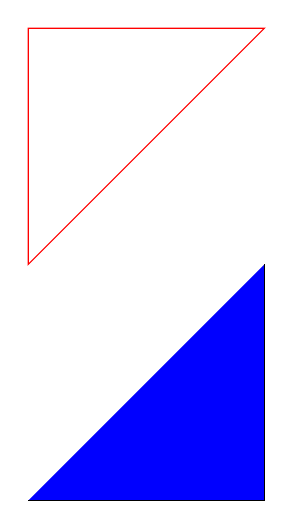
\begin{tikzpicture}[scale=3]
  \draw [fill=blue] (0, 0) -- (1, 0) -- (1, 1);
  \draw [red] (1, 2) -- (0, 2) -- (0, 1) -- cycle;
\end{tikzpicture}
    \caption{Example 1: Vector drawing in TikZ}
  \end{figure}
\end{frame}

\begin{frame}
  \begin{figure}
    \centering
    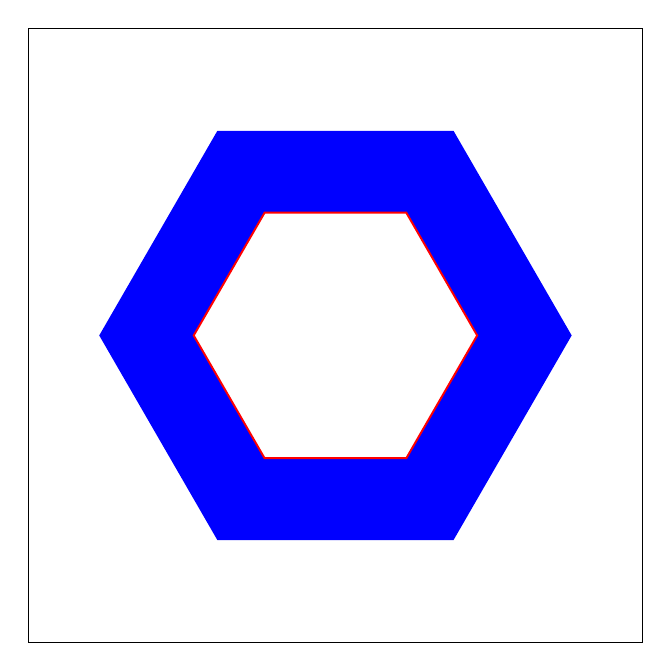
\begin{tikzpicture}[scale=3]
      \draw[line width=0.5pt, black] (-1.3,-1.3) rectangle (1.3,1.3);
      \path[fill=blue, draw=none, even odd rule]
        (0:1) -- (60:1) -- (120:1) -- (180:1) -- (240:1) -- (300:1) -- cycle
        (300:0.6) -- (240:0.6) -- (180:0.6) -- (120:0.6) -- (60:0.6) -- (0:0.6) -- cycle;
      \draw[red, line width=0.7pt]
        (0:0.6) -- (60:0.6) -- (120:0.6) --
        (180:0.6) -- (240:0.6) -- (300:0.6) -- cycle;

    \end{tikzpicture}
    \caption{Task 1: Hexagon drawing}
  \end{figure}
\end{frame}

\begin{frame}
  \begin{figure}
    \center
  \begin{tikzpicture}[scale=3]
    % Don't forget ; in \tikzmath. Even after } .
    \tikzmath{%Do not leave empty lines inside tikzmath. Use comments for visual separation
      \xmin = +1000; \xmax = -1000; \ymin = +1000; \ymax = -1000;
      % \tmin = -pi/2;
      % \tmax =  pi/2;
      % \step = 0.05;
      % tikz expects angles in degrees
      \tmin = -90; % -pi / 2 (* 360 / (2*pi))
      \tmax = 90;
      \step = 0.05 * 180 / pi;
      \a = 1;
      \b = 2;
      %{start, ...increment, end}
      for \t in {\tmin + \step, ...\step,\tmax - \step} {
        \x = \a + \b * cos(\t);
        \y = \a * tan(\t) + \b * sin(\t);
        if \x < \xmin then {
          \xmin = \x;
        };
        if \x > \xmax then {
          \xmax = \x;
        };
        if \y < \ymin then {
          \ymin = \y;
        };
        if \y > \ymax then {
          \ymax = \y;
        };
        %
        \x = \a - \b * cos(\t);
        \y = \a * tan(\t) - \b * sin(\t);
        if \x < \xmin then {
          \xmin = \x;
        };
        if \x > \xmax then {
          \xmax = \x;
        };
        if \y < \ymin then {
          \ymin = \y;
        };
        if \y > \ymax then {
          \ymax = \y;
        };
      };
      \xmax = abs(\xmax);
      \xmin = abs(\xmin);
      \ymax = abs(\ymax);
      \ymin = abs(\ymin);
      if \xmin > \xmax then {
        \xmax = \xmin;
      };
      if \ymin > \ymax then {
        \ymax = \ymin;
      };
      %
      \xmprev = (\a + \b * cos(\tmin + \step)) / \xmax;
      \ymprev = (\a * tan(\tmin + \step) + \b * sin(\tmin + \step)) / \ymax;
      for \t in {\tmin + \step, ...\step,\tmax - \step} {
        \xm = (\a + \b * cos(\t)) / \xmax;
        \ym = (\a * tan(\t) + \b * sin(\t)) / \ymax;
        {\draw[blue] (\xmprev, \ymprev) -- (\xm, \ym);};
        \xmprev = \xm;
        \ymprev = \ym;
      };
      \xmprev = (\a - \b * cos(\tmin + \step)) / \xmax;
      \ymprev = (\a * tan(\tmin + \step) - \b * sin(\tmin + \step)) / \ymax;
      for \t in {\tmin + \step, ...\step,\tmax - \step} {
        \xm = (\a - \b * cos(\t)) / \xmax;
        \ym = (\a * tan(\t) - \b * sin(\t)) / \ymax;
        {\draw[blue] (\xmprev, \ymprev) -- (\xm, \ym);};
        \xmprev = \xm;
        \ymprev = \ym;
      };
    }
  \end{tikzpicture}
  \caption{Example 2.1: Nicomedes' Conchoid}
\end{figure}
\end{frame}

\begin{frame}
  \begin{figure}
    \center
  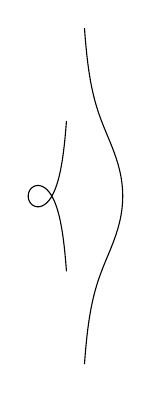
\begin{tikzpicture}
    \def\a{1}
    \def\b{2}
    % {-90+1} so we don't divide by 0. The other +10 are so that we
    % get the picture we want. See the next tikzpicture for a (worse) variant.
    \draw[scale=0.3,domain={-90+11}:{90-11},smooth,variable=\t,samples=180] plot ({\a + \b * cos(\t)}, {\a * tan(\t) + \b * sin(\t)});
    \draw[scale=0.3,domain={-90+11}:{90-11},smooth,variable=\t,samples=180] plot ({\a - \b * cos(\t)}, {\a * tan(\t) - \b * sin(\t)});
  \end{tikzpicture} \hfill
  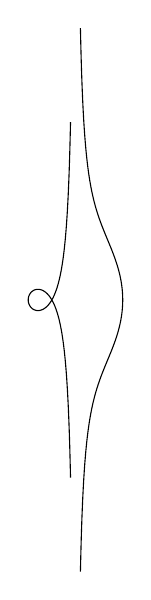
\begin{tikzpicture}
    \def\a{1}
    \def\b{2}
    \draw[scale=0.3,domain={-90+6}:{90-6},smooth,variable=\t,samples=180] plot ({\a + \b * cos(\t)}, {\a * tan(\t) + \b * sin(\t)});
    \draw[scale=0.3,domain={-90+6}:{90-6},smooth,variable=\t,samples=180] plot ({\a - \b * cos(\t)}, {\a * tan(\t) - \b * sin(\t)});
  \end{tikzpicture}
  \caption{Example 2.2: Nicomedes' Conchoid, auto-plot}
\end{figure}
\end{frame}


\begin{frame}
  \begin{figure}
    \center
    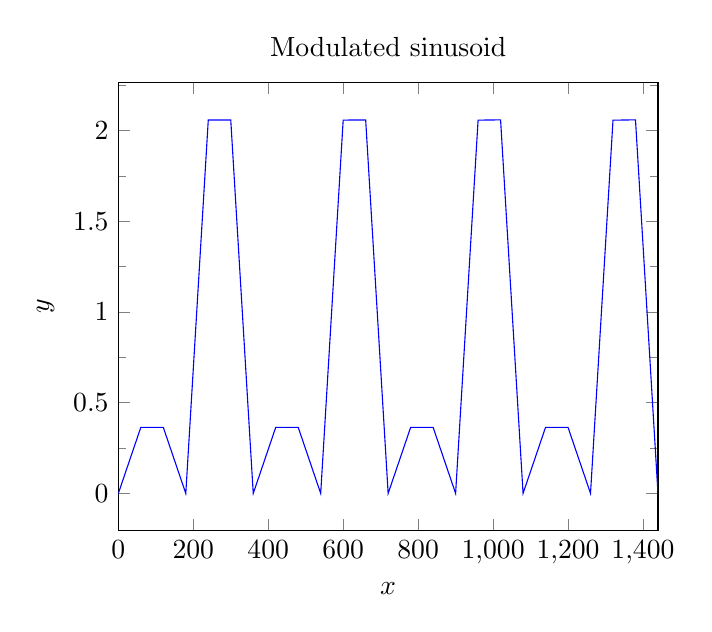
\begin{tikzpicture}
      \begin{axis}[
        title=Modulated sinusoid,
        xlabel={$x$},
        ylabel={$y$},
        domain={0}:{8 * 180}, %8 * pi
        xmin=0, xmax= {8 * 180}, %the actual limits of the plot
        minor y tick num=1, %how many unlabeled ticks between labeled ticks
        ]
        \addplot [blue] {abs(sin(x)) * exp(-sin(x))};
    \end{axis} 
    \end{tikzpicture}
    \caption{Example 2.3: Modulated sinusoid, using PGFPlots. Rough.}
  \end{figure}
\end{frame}

\begin{frame}
  \begin{figure}
    \center
    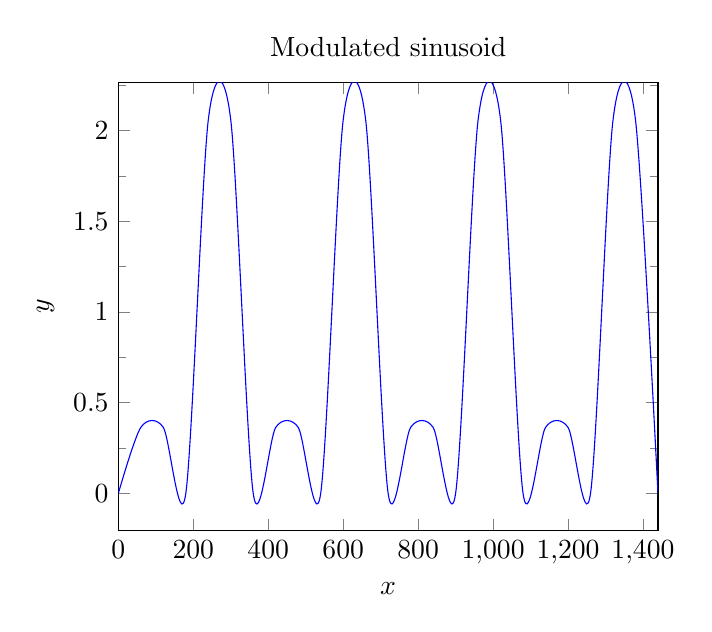
\begin{tikzpicture}
      \begin{axis}[
        title=Modulated sinusoid,
        xlabel={$x$},
        ylabel={$y$},
        domain={0}:{8 * 180}, %8 * pi
        xmin=0, xmax= {8 * 180}, %the actual limits of the plot
        minor y tick num=1, %how many unlabeled ticks between labeled ticks
        smooth,
        ]
        \addplot [blue] {abs(sin(x)) * exp(-sin(x))};
    \end{axis} 
    \end{tikzpicture}
    \caption{Example 2.4: Modulated sinusoid, using PGFPlots. Rough, artificially smoothed.}
  \end{figure}
\end{frame}

\begin{frame}
  \begin{figure}
    \center
    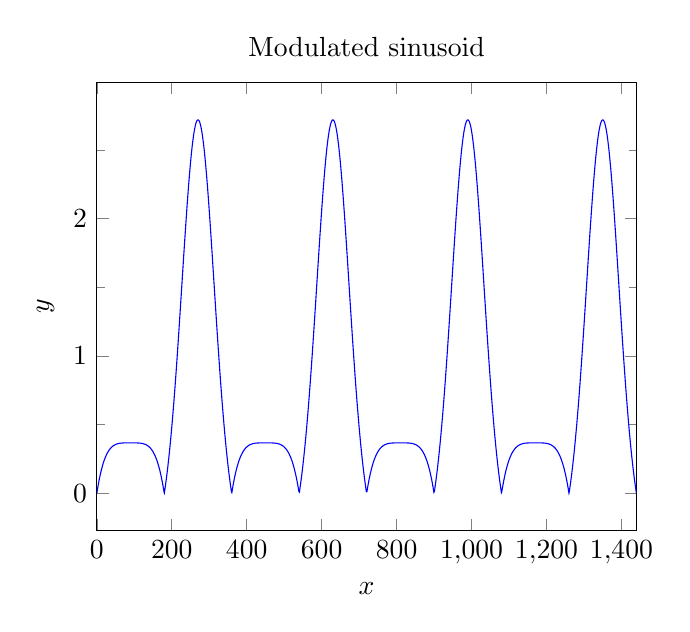
\begin{tikzpicture}
      \begin{axis}[
        title=Modulated sinusoid,
        xlabel={$x$},
        ylabel={$y$},
        domain={0}:{8 * 180}, %8 * pi
        xmin=0, xmax= {8 * 180}, %the actual limits of the plot
        minor y tick num=1, %how many unlabeled ticks between labeled ticks
        smooth,
        samples=1000,
        ]
        \addplot [blue] {abs(sin(x)) * exp(-sin(x))};
    \end{axis} 
    \end{tikzpicture}
    \caption{Example 2.5: Modulated sinusoid, using PGFPlots. Better sampled.}
  \end{figure}
\end{frame}

\begin{frame}
  \begin{figure}
    \centering
    \begin{tikzpicture}[scale=2]
      % Circle Concoid (forma tip limaçon):
      \draw[domain=0:360, samples=400, smooth, variable=\t]
        plot ({(1 + 2*cos(\t)) * cos(\t)},
              {(1 + 2*cos(\t)) * sin(\t)});
    \end{tikzpicture}
    \caption{Task 2: Circle Concoid}
  \end{figure}
\end{frame}



\begin{frame}
\begin{figure}
  \center
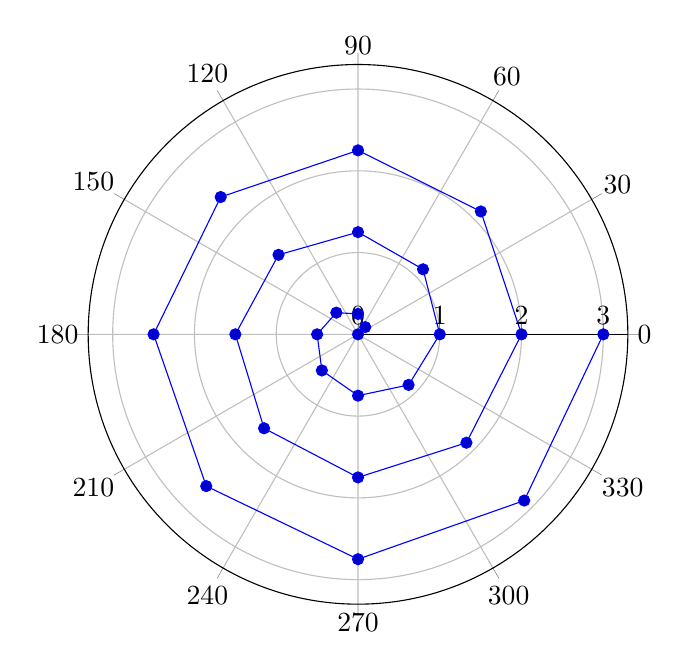
\begin{tikzpicture}
  \begin{polaraxis}
    %try \addplot, notice the difference
    \addplot+ [domain=0:3] (360*x,x); % (angle,radius)
\end{polaraxis} 
\end{tikzpicture}
  \caption{Example 3: Polar plotting}
\end{figure}
\end{frame}

\begin{frame}
  \begin{figure}
    \centering
    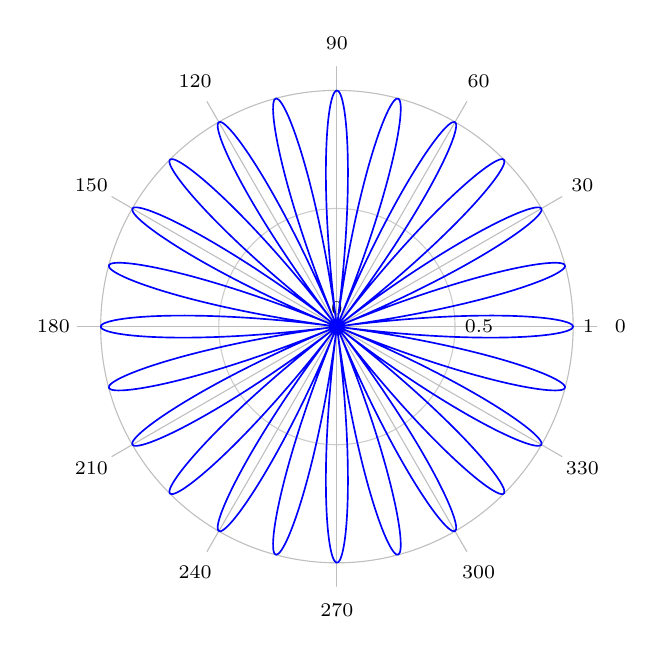
\begin{tikzpicture}[scale=3.0, line cap=round, line join=round]
      
      % --- CERCURI CONCENTRICE ---
      \draw[thin, gray!50] (0,0) circle (1);   % cerc exterior
      \draw[thin, gray!40] (0,0) circle (0.5); % cerc intermediar (raza 0.5)
      
      % --- LINII RADIALE SI ETICHETE UNGHI ---
      \foreach \ang in {0,30,...,330} {
        \draw[thin, gray!50] (0,0) -- (\ang:1.1);
        \node[font=\scriptsize] at (\ang:1.2) {\ang};
      }
      
      % --- ETICHETE PENTRU RAZELE ---
      \node[font=\scriptsize, anchor=west] at (0:0.5) {0.5};
      \node[font=\scriptsize, anchor=west] at (0:1)   {1};
      
      % --- AFISAREA LUI "0" IN CENTRU ---
      \node[font=\scriptsize, anchor=south, yshift=1pt] at (0,0) {0};

      
      % --- CURBA (r = cos(12·θ)) = "Rose curve" ---
      \draw[blue, line width=0.6pt, domain=0:360, samples=720, smooth, variable=\t]
        plot ({cos(12*\t)*cos(\t)}, {cos(12*\t)*sin(\t)});
      
    \end{tikzpicture}
    \caption{Task 3: Polar plotting}
  \end{figure}
\end{frame}

\begin{frame}
  \begin{figure}
    \center
    \begin{tikzpicture}
      \begin{axis} [
        title=Miles per gallon,
        xlabel=hosepower,
        ylabel=mpg,
        ]
        \addplot coordinates {
          (140, 18)
          (140, 17)
          (150, 16)
          (180, 15)
          (220, 14)
        };
        %try removing only marks
        \addplot table [x=horsepower, y=mpg, col sep=comma, only marks] {mpg.csv};
    \end{axis} 
    \end{tikzpicture}
    \caption{Example 4: Plotting datafiles, and coordinates.}
  \end{figure}
\end{frame}



\begin{frame}
  \begin{figure}
    \centering
    \begin{tikzpicture}
      \begin{axis}[
          ymin=0,
          ymax=50,
          xmin=40,
          xmax=220,
          xtick={50,100,150,200},
          ytick={10,20,30,40, 50},
          title={Miles per gallon},
          xlabel={horsepower},
          ylabel={mpg},
        ]
        
        % Blue data points
        \addplot[
          only marks, 
          blue,
          mark=*,
          mark size=1.5pt
        ] table[
          x=horsepower,
          y=mpg,
         col sep=comma
        ] {puncte.csv};
        
        % Red regression line
        \addplot[
          red,
          thick,
          no marks,
          domain=50:200,
          samples=200,
          restrict y to domain=0:40,
          unbounded coords=discard,
        ] {0.00280334*x^2 - 0.9493173*x + 85.533746};
        
      \end{axis}
    \end{tikzpicture}
    \caption{Figure 4: Plotting datafiles. Make sure to clean data, and regress it externally. Here, a $2^{\text{nd}}$ degree polynomial function was fitted in R.}
  \end{figure}
\end{frame}
\end{document}
